\chapter{Introduction}
\section{Motivation}
The main topic of condensed matter physics are about phases and the transitions among them. In particular, to avoid the overshadowing of thermal fluctuations and to reveal the new intricate physics, the zero-temeprature phases and transitions, i.e., the \emph{quantum} phases of matter and \emph{quantum} phase transtions are focused in this thesis.

In fact, the term ``phases'' is never sharply defined like a mathematical concept. It is developing along with the growth of condensed matter physics in the past century. There are two milestones in the development of condensed matter physics: the concept of \emph{Landau fermi liquid} and the phenomena of \emph{spontaneous symmetry breakings}. Landau fermi liquid theory adiabatically connects the interacting electronic fluids with the non-interacting electron gas, with introduction of \emph{quasiparticles} [Landau, Abrikosov]. Quasiparticles has become the most fundenmental object to describe the weakly-interacting systems. This object is so universal that it was believed to constitute our real world at every energy scales. On the other hand, in the pioneering paper of Anderson \cite{anderson1972more}, the philosophy of \emph{emergence} was first proposed, as an declaration on the independence of condensed matter physics, wherein spontaneous symmetry breaking is explained as the fundamental mechanism for the divergent behaviors at different energy scales in different materials.

The most famous and simplest example of the spontaneous symmetry breaking is the 1D transverse-field Ising model
\begin{equation*}
    H=-\sum_{\langle i,j\rangle}J\sigma_i^z\sigma_j^z-h\sum_i\sigma_i^x,
\end{equation*}
which is clearly invariant under the $\mathbb Z_2$ spin flip transformation: $\sigma_z\rightarrow-\sigma_z$. However, when looking at the gound states, clearly at small external field $h\ll J$ the ground state will be ferrormagnetic, where all spin align to $\hat z$ or $-\hat z$ direction to minimize the energy, explicitly breaking the $\mathbb Z_2$ symmetry of the Hamiltonian. While at large external field $h\gg J$, the ground state will be polarized along the $\hat x$ direction, restoring such $\mathbb Z_2$ symmetry.

% is really not a new concept: it occurs everyday in our normal life. Taking water as the example, as a normal fluid it is continuously translational-invariant and isotropic, or has $\mathbb R^3\times\mathrm{O}(3)$ symmetry in the language of group theory. When cooling down below the freezing point, solid ice will be formed, leaving just discrete translation symmetry and discrete rotation symmetries.


Due to the early success in explanation of Fermi liquid \cite{landau1959theory}, He-II superfluidity \cite{landau1941theory}, and BCS superconductivity \cite{bardeen1957theory,bardeen1957microscopic}, it has been a long time for people to believe that the combined paradigm of Landau fermi liquid theory (particularly with the concept of quasiparticles) and the mechanism of spontaneous symmetry breaking, tells the whole story of condensed matter physics. Moreover, with the help of renormalization group (RG) analysis, people at that time even tends to believe that everything in condensed matter physics is predictable, as long as the quasiparticle properties and system symmetries are known.

However, nowadays we know the story came to totally different endings: the subsequntly discoveries of unconventional high-$T_c$ superconductivity beyong BCS theory, from cuprates \cite{bednorz1986possible}, to iron-based superconductors \cite{kamihara2006iron} and Nickel-based superconductors \cite{li2019superconductivity}, from bulk materials like YBCO [] and BiSSCO [] to thin-film materials like monolayer FeSe \cite{liu2012electronic} and twisted bilayer graphene (tBLG) \cite{cao2018correlated,cao2018unconventional}, have all provided the evidence for the breakdown of quasiparticle pictures. And the discoveries of integer quantum Hall effect (IQHE) \cite{klitzing1980new} and fractional quantum Hall effect (FQHE) \cite{tsui1982two,willett1987observation}, together with the following proposals and realizations on the huge family of topological insulators (TI) \cite{bernevig2006quantum,hsieh2008topological} and topological superconductors \cite{xu2014artificial}, have all revealed the importance of \emph{topology} in condensed matter physics, which has been longly overlooked by the traditional paradigm of Landau fermi liquid thoery plus spontaneous symmetry breakings. Particularly, nowadays \emph{topological orders} \cite{wen1990topological,levin2005string,chen2010local,wen2002quantum}, first proposed by Wen in understanding of the ground state degeneracy in FQHE \cite{wen1990ground}, has become the fundamental language in describing and classification of quantum states of matter. And the interplay between topological orders (either trivial or not) and \emph{symmetries} has been further developed into a vast framework classifying all quatum phases of matter in our universe, including \emph{symmetry-protected topological trivial states (SPT)} \cite{chen2013symmetry} and \emph{symmetry-enriched topological orders states (SET)} \cite{mesaros2013classification}.


\section{Outline of the Thesis}
It can be seen that the very-beginning ``featureless'' concept of phases in condensed matter physics has been highly complexified (and classified) due to the interplay of symmetry, topology, and strong-correlations. In this thesis, I will focus on the study of the quantum phases of matter in two-dimensional space, particularly in the context of the \emph{twisted} 2D materials exhibiting all these complexities. The thesis is organized as follows:
\begin{itemize}
    \item In the beginning, I will generally introduce the complexity brought by dimensionality (particularly 2D), symmetry and topology. To explain the new tunable knob of \emph{twistings}, I will take graphene and transition metal dichalcogenides as two typical examples of 2D materials to introduce the \emph{moir\'{e} physics}.
    \item As the main part of the thesis, I will list three of my works on twisted 2D materials. The former two works are about twisted 2D superconductors, where complexities of free-fermion topology and symmetries get involved. The other recent long work is for \emph{fractional Chern insulators} (FCI), the lattice analogue of FQHE, realized in twisted transition metal dichalcogenides. In construction of the framework, all factors of complexity mentioned above get intertwined, including moir\'{e} physics, strong correlations, and symmetry-enriched topological orders.
\end{itemize}

% \section{Complexity from Dimensionality: 2D}
% In this section, I will briefly discuss the complexity of the condensed matter systems from the perspective of dimensionality. Particularly, I will focus on the two-dimensional systems, as it is the main topic of this thesis. \textbf{[todo!]}
% \begin{itemize}
%     \item \textbf{Statistics in 2D: Anyons.} The most famous example exhibiting the particularity of the two-dimensional space is on the classification of elementary particles. The modern thoery explaining the statistics of elementary particles is to consider the \emph{dynamic process of braiding} \cite{laidlaw1971feynman,wu1984general}. In path-integral formalism, it is
%           \begin{equation*}
%               _f\langle \{\bm x_N\}|\{\bm x_N\}\rangle_i\equiv\int_{\gamma}\mathcal D\{\bm x_N\}\, e^{iS[\{\bm x_N\}]}=\sum_{[\gamma]\in\pi_1(M_N)}\chi([\gamma])\int_{\gamma\in[\gamma]}\mathcal D\{\bm x_N\}\, e^{iS[\{\bm x_N\}]}.
%           \end{equation*}
%           Here we sum up all paths $\gamma\in M_N$ of the configuration space $M_N$ connecting the initial/final states. We further grouped them into topologically inequivalent sectors, classified by the first homotopy class $\pi_1(M_N)$.

%           Clearly $M_N\subset\mathbb R^{Nd}=\mathbb R^d\times\cdots\times\mathbb R^d$ is the subspace of the full $N$-particle configuration space. Now because we are interested in the braiding processes only, all the trivial configurations that have particles occupying the same positions $\Delta=\{(\bm x_1,\cdots,\bm x_N)|\exists i\neq j, \bm x_i=\bm x_j\}$ should be excluded. Due to the indistinguishability of $N$-particles, any mutual exchange (relabeling) of particles described by the permutation group $S_N$ should be considered as the same configuration . As a result, the configuration space $M_N=(\mathbb R^{Nd}\backslash \Delta)/S_N$. Depending on the spatial-dimensionality, we have the following results \cite{wu1984general}:
%           \begin{itemize}
%               \item In $d=1$: there is no sense to talk about braiding operations.
%               \item In $d=2$: $\pi_1(M_N)=B_N\equiv\langle\sigma_1\cdots\sigma_{n-1}|\sigma_i\sigma_j=\sigma_j\sigma_i,\sigma_i \sigma_{i+1}\sigma_i=\sigma_{i+1}\sigma_i \sigma_{i+1}\rangle$ is the \emph{braid group}.
%               \item In $d\geq3$: $\pi_1(M_N)=S_N\equiv\langle\sigma_1\cdots\sigma_{n-1}|\sigma_i^2=1,\sigma_i\sigma_j=\sigma_j\sigma_i,\sigma_i \sigma_{i+1}\sigma_i=\sigma_{i+1}\sigma_i \sigma_{i+1}\rangle$ is the \emph{permutation group}.
%           \end{itemize}
%           For one-dimension representations $\rho:\sigma_i\mapsto e^{i\theta_i}$, the presentation constraints shared by $S_N$ and $B_N$ simply tells $\theta_i=\theta_{i+1}=\theta$. Relation $\sigma_i^2=1$ in $S_N$ futher fixes $\theta=0,\pi$, or weight $\chi_\pm([\alpha])=\pm1$ as the sign of the permutations, explaining the \emph{spin-statistics theorem} or the origin of bosons/fermions in $(3+1)$-d field theory. For braid group, however, $\chi_\theta([\alpha])=e^{i\theta}$ can be chosen arbitrarily. Each abelian representation $\chi_\theta$ corresponds to one \emph{abelian anyons} \cite{wilczek1982quantum}.

%           The above argument \emph{implicitly assume that the Hilbert space of a collection of particles at specified positions is one-dimensional}. If we release that assumption by considering a many-particle state with extra $\mathcal D$-degeneracy (the \emph{total quantum dimension} \cite{kitaev2006topological,levin2006detecting}) apart from the degeneracy in conventional sense such as single-particle's spin/flavor/valley/band indices, then the amplitude between the initial/final states becomes
%           \begin{equation*}
%               _f\langle\{\bm x_N\},n|\{\bm x_N\},n'\rangle_i=\sum_{[\gamma]\in\pi_1(M)}\chi_{nn'}([\gamma])\int_{\gamma\in[\gamma]}\mathcal D\{\bm x_N\}\, e^{iS[\{\bm x_N\}]},
%           \end{equation*}
%           where $\mathcal D$-dimensional non-abelian representation $\chi:\pi_1(M_N)\rightarrow\mathrm{GL}_{\mathcal D}(V)$ enters. In two-dimensional space, $\chi: B_N\rightarrow\mathrm{GL}_{\mathcal D}(V)$ gives the classification of \emph{non-abelian anyons}\footnote{The \emph{parastatistics}, named for non-abelian representation of higher dimensional space, though exits in mathematical sense, is excluded in the path integral formalism in the long proof of Ref. \cite{laidlaw1971feynman}}. Besisdes the non-abelian mutual statistics, there is another intrinsic property called the \emph{fusion rules} $\phi_a\star\phi_b=\sum_c N^c_{ab}\phi_c$ by considering the composite particle . As an appreciation of the complexity in 2D, it is enough to pause the discussion here.

%     \item \textbf{Disorder in 2D: Weak Localization.} In the seminal paper by ``the gang of four'' Abrahams, Anderson, Licciardello, and Ramakrishnan in Ref. \cite{abrahams1979scaling}, a scaling theory is constructed with the strong hypothesis that the change of the conductance $G$ with the length scale $L$ depends solely on the conductance at previous length scales, and not, for example, independently on $L$ or on the strength of the disorder. The RG equation for the conductance is then a single-parameter scaling equation
%           \begin{equation*}
%               \dfrac{\mathrm d\ln G}{\mathrm d\ln L}=\beta(G(L)).
%           \end{equation*}
%           In the weak disorder limit $G\gg1$ where Ohm's law is expected to hold (or microscopically the diffusive Drude physics dominates), the conductance $G=1/R=\sigma\frac{L}{A}\sim\sigma L^{2-d}$, giving
%           \begin{equation*}
%               \lim_{\ln G\rightarrow\infty}\beta(G)=d-2.
%           \end{equation*}
%           While in the strong disorder limit $G\ll1$ where Anderson's strong-disorder perturbation thory [] holds, and the conductance should drop off exponentially with the system size $G(L)=G_0 e^{-L/\xi}$, or
%           \begin{equation*}
%               \lim_{\ln G\rightarrow-\infty}\beta(G)=-\frac{L}{\xi}\simeq\ln G\rightarrow-\infty.
%           \end{equation*}
%           Naive smooth connection of these two limit regimes tells that (see Fig. \ref{fig:scaling_of_Anderson_localization})
%           \begin{itemize}
%               \item In $d=1$: $\beta(G)<0$ and the system will always flow to the insulating regime.
%               \item In $d=2$: marginal case.
%               \item In $d=3$: there is one critical point $G_c$ above which the system will flow to the metallic regime, and below which the system will flow to the insulating regime.
%           \end{itemize}
%           \begin{figure}[!htp]
%               \centering
%               \includegraphics[width=0.7\textwidth]{figures/scaling_of_Anderson_localization.pdf}
%               \caption{Schematic Plot on the RG Flow of the Conductance}
%               \label{fig:scaling_of_Anderson_localization}
%           \end{figure}
% \end{itemize}

% \section{Complexity from Symmetry and Topology}
% Modern classification theory on quantum phases of matter is based on the intrinsic property of the quantum states: quantum entanglement. The concept of \emph{local unitary transformation} (LU) was proposed first in classificaltion of the matrix product states representation of the 1D gapped spin systems
% \begin{equation*}
%     |\Psi\rangle=\sum_{s_1,\cdots,s_N}\mathop{\mathrm{Tr}}\bigg[A_1^{s_1}A_2^{(s_2)}\cdots A_N^{(s_N)}\bigg]|s_1,s_2,\cdots,s_N\rangle,
% \end{equation*}
% by Chen, Gu and Wen in \cite{chen2011classification} . They quickly realize that the framework of LU can be generalized to other quantum phases in \cite{chen2010local}, resulting in the famous map:

% \subsection{Free fermion Topology: Example of 10-fold Way}
% The key feature of SPT state is the presence of the \emph{gapless} edge states that are protected by the symmetry. Namely we


% \subsection{Symmetry Enrichment: SPT and SET}
% Symmetry protected topological (SPT) order exists in gapped systems with global symmetry. The ground state of the system does not spontaneously break the symmetry, has no fractional excitation, yet cannot be smoothly connected to a product state without explicitly breaking the symmetry. The nontrivial natural of the SPT order can be manifested in two ways:
% \begin{enumerate}
%     \item As nontrivial edge states which must either be gapless, spontaneously break symmetry or support anomalous SF pattern (with bulk dimension $\geq3$) as long as the global symmetry is not explicitly broken.
%     \item For SPT phases with unitary on-site symmetry, gauging the symmetry results in nontrivial gauge theories whose gauge fluxes have nontrivial braiding statistics.
% \end{enumerate}

% It was shown that a large class of SPT phases in boson/spin systems in dimension d has a one to one correspondence with equivalence classes of group cocycles $H^{d+1}(G, U (1))$ [Witten]. For unitary G, gauging the symmetry results in $d$ dimensional Dijkgraaf-Witten (DW) gauge theory characterized also by the equivalence class of cocycles []. For example, the double semion theory in 2D is a DW gauge theory of gauge group $\mathbb Z_2$ corresponding to the nontrivial element in $H^3 (\mathbb Z_2 , U(1))$. For definition of group cocycles and discussion of their relation with SPTs and gauge theories , see Refs. [].
% For the discussion in this review, it suffices to know that the set of equivalence classes of group cocycles in $H^{d+1}(G, U (1))$ forms an abelian group. For $d=0$, elements in $H^1(G, U(1))$ corresponds to one dimensional representations of $G$ which have a one to one correspondence with symmetry charges of $G$. For $d=1$, elements in $H^2(G, U(1))$ corresponds to projective representations of $G$ with $U(1)$ coefficient; such projective representations are realized as degenerate edge states of one dimensional SPT phases. We collect a few simple mathematical results of $H^{d+1}(G, U (1))$, for $d\geq1$, ...


\section{Complexity from Twisting: Moir\'{e} Physics}
\subsection{2D Materials}
\subsubsection{Graphene}
Historically, there exists many arguments claiming the non-existence of 2D materials due to the instability under finite thermal fluctuations\footnote{For example, a naive (so \emph{wrong}) entropy argument goes as following: Note that 2D material has less vibration modes than 3D materials of the same particle number, the entropy contribution from these vibration modes should be smaller in 2D, so is not entropy-favored.}, and even Lev Landau made mistakes here\footnote{Landau claim the non-existence based on the experimental facts that no divergence has been observed under a disorder to order (like liquid to crystal) phase transition.}. All of these arguments are disputed by the discovery of graphene in 2004 by Geim and Novoselov \cite{novoselov2004electric}. And the realistic two-dimensional world has been opened since then.

Graphene is well-known for the presence of Dirac points in its band structure. For the honeycomb lattice constituted of carbon atoms only, there exists sublattice (inversion) symmetry between $A,B$ sites. For spinless electrons, where Hamiltonian is written in such pseudospin basis as a general two-by-two matrix $H(\bm k)=\bm d(\bm k)\cdot\bm \tau$ with real vector coefficients $\bm d(\bm k)$, the inversion operator $\mathcal P$ exchanging $A,B$ sites can be represented as $P=\tau_x$. Graphene also possesses time-reversal symmetry, and for spinless electrons the time-reversal operator is simply a complex conjugate $T=K$. Therefore, the combination of inversion symmetry and time-reversal symmetry keeping the momentum unchanged: $\mathcal P\mathcal T:\bm k\mapsto\bm k$, requires the Hamiltonian to satisfy
\begin{equation*}
    \tau_x^{-1}H^*(\bm k)\tau_x=H(\bm k),
\end{equation*}
implying $d_3(\bm k)=0$ or $H(\bm k)=d_1(\bm k)\tau_x+d_2(\bm k)\tau_y$ with ALL matrix element off-diagonal. Now because both the momentum and the Hamiltonian share the same dimensionality, given one zero solution of the eigen equation $\det|\lambda I-H(\bm k)|=0$, any perturbation preserving the inversion and time-reversal symmetries, i.e., constituted of $\tau_x$ and $\tau_y$ matrices, cannot destroy such zero point. That is the typical example of symmetry-protected Dirac points (if exists) in graphene.

To obtain the low-energy description of graphene, we can implement the spatial $C_3$ rotation symmetry to the Hamiltonian
\begin{equation}\label{eq:C3 rotation constraint}
    C_3^{-1}H(\bm k)C_3=H(\mathcal C_3^{-1}\bm k).
\end{equation}
\noindent Precisely speaking, we can expand the general Hamiltonian around $K$ and $K'$ to the lowest linear-order
\begin{equation*}
    d_1(\bm k)=a_{10}+a_{11}k_x+a_{12}k_y,\quad d_2(\bm k)=a_{20}+a_{21}k_x+a_{22}k_y
\end{equation*}
or
\begin{equation*}
    H(\bm k)=\begin{pmatrix}
                                                                 & (a_{10}-ia_{20})+(a_{11}-ia_{21})k_x+(a_{12}-ia_{22})k_y \\
        (a_{10}+ia_{20})+(a_{11}+ia_{21})k_x+(a_{12}+ia_{22})k_y &
    \end{pmatrix}
\end{equation*}
and insert back to the constraint Eq. \eqref{eq:C3 rotation constraint}. One gets
\begin{equation*}
    a_{31}=a_{32}=0,\quad a_{10}=a_{20}=0,\quad a_{12}=-a_{21},\quad a_{11}=a_{22},
\end{equation*}
and we end up with the well-known Dirac cone Hamiltonian
\begin{equation}
    H_K(\bm k)=\hbar v_F\bm k\cdot\bm\tau\equiv\hbar v_F|\bm k|\left(\begin{array}{cc}
                      & e^{-i\theta_k} \\
        e^{i\theta_k} &
    \end{array}\right)
\end{equation}
with the angle of the momentum $\theta_k\equiv\arctan\frac{k_y}{k_x}$.

\subsubsection{Transition Metal Dichalcogenides (TMDs)}
Apart from the typical example of graphene, there are also growing interests in other atomically thin 2D material for their potential application in next-generation of nano devices. In particular, due to its easy fabrication on mechanical exfoliation, transition-metal dichalcogenides (TMD) stands out as the most promising representatives.



TMDs of chemical formula MX$_2$, typically comprise a plane having hexagonally-placed transition metal atoms M (group-IIIB to group-IIB) placed between two chalcogen atom-based hexagonal planes X (e.g., S, Se, Te). There are three monolayer structures: the \emph{trigonal prismatic} 1H phase, the \emph{distorted octahedral} 1T phase, and the \emph{dimerized} 1T' phase, as are shown in Fig. \ref{fig:TMD_electonic_properties}.
\begin{figure}[!htp]
    \centering
    \includegraphics[width=1.0\textwidth]{figures/TMD.png}
    \caption{\textbf{Structure and electronic properties of TMDs} adapted from Ref. \cite{manzeli20172d}. \textbf{(a)} Atomic structure of single layers of TMD in their \emph{trigonal prismatic} (2H), \emph{distorted octahedral} (1T) and \emph{dimerized} (1T') phases. \textbf{(b)} ``Periodic table'' of known layered TMDs, organized based on the transition metal elements, their existing structural phases (2H, 1T and 1T'), and the observed electronic phases (see the right panel). \textbf{(c)} Evolution of the band structure of 2H-MoS$_2$ from bulk material down to monolayers. Clearly a indirect gap to direct gap transition occurs for monolayer material only. \textbf{(d)} Schematic band structure of 2H-MoS$_2$, showing the spin splitting (orange and blue colors) at K and K' points.)}
    \label{fig:TMD_electonic_properties}
\end{figure}
We will mostly focus on the group V and group VI transition metal elements, particularly those with 1T and 1T' phases shown to be unstable. So without loss of generalization, when we talk about monolayer TMDs in this thesis, we always refer to the 1H phase structure.
% \begin{figure}[!htp]
%     \centering
%     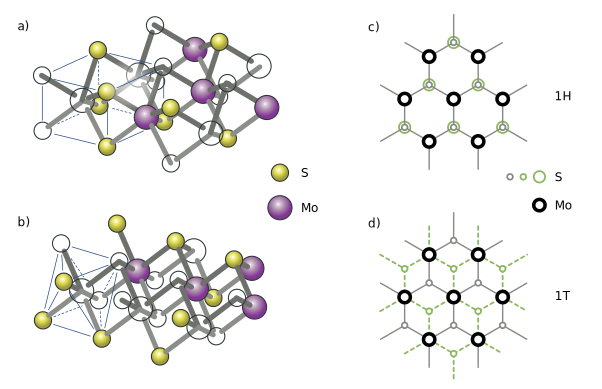
\includegraphics[width=0.8\textwidth]{figures/MoTe2_crystal_structure.pdf}
%     \caption{\textbf{Monolayer $\mathrm{MoS_2}$} (extracted from \url{https://en.wikipedia.org/wiki/Transition_metal_dichalcogenide_monolayers}). a) and c) for 1H phase of monolayer $\mathrm{MoS_2}$, and b) and d) for 1T phase of $\mathrm{MoS_2}$, which is \emph{metastable}. c) and d) are schematic top views, respectively. The 1H ground state has prismatic structure of chalcogen atoms surrounding the transition metal atoms, and the top/bottom layer of chalcogen atoms are the same. The metastable 1T phase shows octahedral structure, less relevant to our discussion, can be viewed by rotating all chalcogen atoms on the top layer by 30 degrees with respect to the lower layers.}
%     \label{fig:MoTe2_crystal_structure}
% \end{figure}
% The 1T phase is \emph{metastable} and is NOT relevant to our discussion. 


For monolayer TMDs of 1H phase, the corresponding bulk material are mostly of 2H stacking form, with \emph{alternating} alignment of transition metal atoms and chalcogen atoms, as is shown in (a) in Fig. \ref{fig:MoS2_Di}.
\begin{figure}[!htp]
    \centering
    \includegraphics[width=0.8\textwidth]{figures/MoS2_Di.png}
    \caption{\textbf{MoS$_2$ Crystal Structure and Band Structure} adapted from Ref. \cite{xiao2012coupled}. \textbf{(a)} The unit cell of bulk 2H-MoS$_2$. \textbf{(b)} Top view of MoS$_2$ monolayer. \textbf{(c)} Schematic drawing of the band structure at the band edges located at the K points.}
    \label{fig:MoS2_Di}
\end{figure}
Experimentally, there has been reports on the emergence of the peak in the optical spectroscopy study in Ref. \cite{mak2010atomically} and photoluminescence (PL) signals in Ref. \cite{splendiani2010emerging}, which is ascribed as the manifestation on the evolution of of the TMD band structure from bulk's indirect gap to monolayer's direct $K$-$K$ gaps, see (c) in Fig. \ref{fig:TMD_electonic_properties}.

Taking group-IV dichalcogenides MX$_2$ as the example, the 2H stacking bulk material has space group $D_{6h}$ with inversion symmetry (see (a) in Fig. \ref{fig:MoS2_Di}), but reduces to $D_{3h}$ breaking the inversion symmetry down to monolayers. For monolayer MX$_2$, DFT calculation tells that the relevant orbitals within the conduction and valence bands around $K$ and $K'$ points are mostly from d-orbitals \cite{mattheiss1973band}. From the character table of $D_{3h}$ (see, for example, \url{http://symmetry.jacobs-university.de/cgi-bin/group.cgi?group=603&option=4})
% \begin{table}[htp!]
%     \centering
%     \begin{tabular}{|c|c|c|c|c|c|c|c|c|}
%         \hline\hline
%         $\mathbf{D_{3h}}$ & $E$  & $2C_3$ & $3C_2'$ & $\sigma_h$ & $2S_3$ & $3\sigma_v$ & linear  & quadratic        \\ \hline\hline
%         $A_1'$            & $+1$ & $+1$   & $+1$    & $+1$       & $+1$   & $+1$        &         & $x^2+y^2$, $z^2$ \\ \hline
%         $A_2'$            & $+1$ & $+1$   & $-1$    & $+1$       & $+1$   & $+1$        &         &                  \\ \hline
%         $E'$              & $+2$ & $-1$   & $0$     & $+2$       & $-1$   & $0$         & $(x,y)$ & $(x^2-y^2,xy)$   \\ \hline
%         $A_1''$           & $+1$ & $+1$   & $+1$    & $-1$       & $-1$   & $-1$        &         &                  \\ \hline
%         $A_2''$           & $+1$ & $+1$   & $-1$    & $-1$       & $-1$   & $+1$        & $z$     &                  \\ \hline
%         $E''$             & $+2$ & $-1$   & $0$     & $-2$       & $+1$   & $0$         &         & $(xz,yz)$        \\ \hline
%     \end{tabular}
%     \caption{\textbf{Character Table of $D_{3h}$ Group}.}
%     \label{tab:Character Table of D3h Group}
% \end{table}
we know that the trigonal prismatic crystal field splits the d-orbitals of transition metal elements into three groups: $A_1'(d_{z^2})$, $E'(d_{xy}, d_{x^2-y^2})$, and $E''(d_{xz}, d_{yz})$, where the former two groups $A_1'$ and $E'$ is even under the in-plane mirror symmetry $\sigma_h: z\rightarrow-z$, while the latter one $E''$ is odd under $\sigma_h$. Now that only two bands are concerned in our analaysis: the conduction band and the valence band, we can simply take the irreps $A_1'$ and $E'$ into account, resulting in a simple two-band model $H_\tau(\bm k)=\bm d(\bm k)\cdot\bm\sigma$ if the spin-orbit coupling is temporarily ignored.

To the lowest-order expansion, the constant part of the diagonal terms represent the $K$-$K$ (or $K'$-$K'$) direct band gap $\Delta$. While for the off-diagonal term, we can either use the brute-force expansion and fix the expansion coefficients using $C_3$ rotation transformation as we did for graphene, or use the standard $\bm k\cdot\bm p$ analysis \cite{dresselhaus1955spin,voon2009kp,kormanyos2015k} by computing the matrix element $\langle \psi_a|\frac{\hbar}{m}\bm k\cdot\hat{\bm p}|\psi_b\rangle$ for $|\psi_{a,b}\rangle\in\{|\psi_{A_1'}\rangle,|\psi_{E'}\rangle\}$. Note: not all terms survives in such matrix element. In fact, because we have the rotation eigenvalues $C_3|\psi_{A_1'}\rangle=|\psi_{A_1'}\rangle$ and $C_3|\psi_{E'}\rangle=e^{i\frac{2\pi}{3}}|\psi_{E'}\rangle$ (for $K$-valley, for example), and for $\hat p_\pm\equiv\hat p_x\pm i \hat p_y$ we have $C_3\hat p_\pm C_3^\dagger=e^{i\mp\frac{2\pi}{3}}$, the $C_3$ rotation tansformation forces either term within $H_{\bm k\cdot\bm p}\equiv\frac{\hbar}{2m}\bm k\cdot\hat{\bm p}\equiv\frac{\hbar}{2m}(k_+\hat p_- + k_-\hat p_+)$ to be vanishing in the off-diagonal matrix element, leaving simply the massive Dirac Hamiltonian (with insertion of valley index)
\begin{equation}
    H_{\text{eff}}^{\text{SOC off}}=H_0+H_{\bm k\cdot\bm p}=\begin{pmatrix}
        \frac{\Delta}{2} & Ak_-              \\
        Bk_+             & -\frac{\Delta}{2}
    \end{pmatrix}\equiv\hbar v_F(\tau k_x\sigma_x+k_y\sigma_y)+\frac{\Delta}{2}\sigma_z.
\end{equation}

Now let us include the spin-orbit couplings (SOC) in the $\bm k\cdot\bm p$ analaysis
\begin{equation*}
    H_{\bm k\cdot\bm\pi}\equiv\frac{\hbar}{m}\bm k\cdot\left(\bm p+\frac{\hbar}{4mc^2}\bm s\times\nabla V\right).
\end{equation*}
The SOC Hamiltonian can also be written as $H_{\text{SOC}}=\lambda\bm L\cdot\bm  s=\lambda(L_z s_z + L_+  s_- + L_-  s_+)$. Noting that both $L_+$ and $L_-$ are odd under in-plane mirror symmetry $\sigma_h$, while $L_z$ is even, so the orbital-part of the matrix element satisfying $\langle\psi_a|L_\pm|\psi_b\rangle\equiv\langle\psi_a| s_h^{-1}  s_h L_\pm s_h^{-1} s_h|\psi_b\rangle$ must connect states whose orbital contents behaves \emph{differently} under $\sigma_h$. However, our chosen basis $|\psi_{A_1'}\rangle$ and $|\psi_{E'}\rangle$ are both even under $\sigma_h$, so we are left with simply the $L_z$ term, resulting
\begin{equation}
    H_{\text{eff}}=H_0+H_{\bm k\cdot\bm\pi}=H_{\text{eff}}^{\text{SOC off}}\otimes s_0 + \begin{pmatrix}
        \Delta_{A_1'\text{-SOC}} &                        \\
                                 & \Delta_{E'\text{-SOC}}
    \end{pmatrix}\otimes s_z
\end{equation}
with $\Delta_{A_1'\text{-SOC}}$ and $\Delta_{E'\text{-SOC}}$ dictating the band splittings due to SOC. The energy scale of them can be read from the DFT results in Fig. \ref{fig:monolayer_TMD_band_structure},
\begin{figure}[!htp]
    \centering
    \includegraphics[width=0.9\textwidth]{figures/monolayer_TMD_band_structure.png}
    \caption{\textbf{DFT Band Structures for Several MX$_2$ Monolayer Materials} (extracted from \cite{ramasubramaniam2012large}).}
    \label{fig:monolayer_TMD_band_structure}
\end{figure}
where $\Delta_{A_1'\text{-SOC}}$ always turns out to be almost vanishing so we jut ignore it. The final form of the effective Hamiltonian (with insertion of valley index)
\begin{equation}\label{eq:MoS2 kdotp}
    H_{\text{eff}}=\bigg(\hbar v_F(\tau k_x\sigma_x+k_y\sigma_y)+\frac{\Delta}{2}\sigma_z\bigg)\otimes s_0 - \lambda\tau\frac{\sigma_z-\mathbf 1}{2}\otimes s_z.
\end{equation}


\subsection{Twisting with Moir\'{e} Physics}
Moir\'e patterns are known as the interference patterns generated when two or more periodic structures of the same scale (lattice constant $a$) are overlaid. The interference pattern exhibits a new large-scale (coin as \emph{Moir\'{e} scale}) periodic structure on top of the original one (which can be different from the original ones), so that the original lattice information is smeared out, leaving physics occurring at such new Moir\'{e} scale.

The general bilayer system can be described with two set of grids spanned by $\{\bm R_{l,1},\bm R_{l,2}\}$ with $l=1,2$ labeling the layers. We are interested in the physics when the two layers are related with some rotation $\mathcal R_\theta$  and some displacement $\bm d$. Namely the same cartesian coordinate within these two coordinates systems are related with the linear transformation: $\bm{r}_{l',\alpha}=\mathcal R_\theta\bm{r}_{l,\alpha}+\bm d$. This leads to to a useful identity for the inner product that
\begin{equation}\label{eq:twisted dot product}
    \bm k_{l'}\cdot\bm r_{l',\alpha}\equiv(\mathcal R_\theta\bm k_l)\cdot(\mathcal R_\theta\bm r_{l,\alpha}+\bm d)\equiv\bm k_l\cdot\bm r_{l,\alpha}+\bm k_l\cdot\bm d,
\end{equation}
where we recognize $\bm k_l\equiv\mathcal R_\theta\bm k_{l'}$.

Each layer possesses its own Bloch states
\begin{equation*}
    |\bm k_l,\alpha\rangle =\dfrac{1}{\sqrt N}\sum_{\bm R_l} e^{i\bm k_l\cdot(\bm R_l+\bm\tau_{l,\alpha})}|\bm R_l+\bm\tau_{l,\alpha}\rangle,
\end{equation*}
so the general momentum-space Hamiltonian of the bilayer system can be obtained from the matrix element
\begin{align*}
    \langle\bm k_l,\alpha|H|\bm k'_{l'},\alpha'\rangle & =\frac{1}{N}\sum_{\bm R_l,\bm R'_{l'}}e^{-i\bm k_l\cdot(\bm R_l+\bm\tau_{l,\alpha})}e^{i\bm k'_{l'}\cdot(\bm R'_{l'}+\bm\tau_{l',\alpha'})}\langle\bm R_l+\bm\tau_{l,\alpha}|H|\bm R'_{l'}+\bm\tau_{l',\alpha'}\rangle.
\end{align*}
Since the Wannier center is highly localized in real-space, it is OK to take the real-space matrix element on the right hand side as a function of the distance of two Wannier centers only (and of course also labelled with the species of the Wannier orbitals), i.e.
\begin{equation*}
    \langle\bm R_l+\bm\tau_{l,\alpha}|H|\bm R'_{l'}+\bm\tau_{l',\alpha'}\rangle\simeq H_{l,\alpha;l',\alpha'}(\bm R_l+\bm\tau_{l,\alpha}-\bm R'_{l'}-\bm\tau_{l',\alpha'})
\end{equation*}
know as the \emph{two-center approximation} \cite{bistritzer2011moire}. Scalar function $H(\bm R_l+\bm\tau_{l,\alpha}-\bm R'_{l'}-\bm\tau_{l',\alpha'})$ is still periodic. Switching to momentum space, and using the Poisson summation formula
\begin{equation*}
    \frac{1}{N}\sum_{\bm R}e^{i\bm R\cdot\bm q}=\sum_{\bm G}\mathcal F[e^{i\bm R\cdot\bm q}](\bm G)=\sum_{\bm G}\delta_{\bm q,\bm G}
\end{equation*}
we have
\begin{align}
    \langle\bm k_l,\alpha|H|\bm k'_{l'},\alpha'\rangle & =\frac{1}{N}\sum_{\bm R_l,\bm R'_{l'}}e^{-i\bm k\cdot(\bm R_l+\bm\tau_{l,\alpha})}e^{i\bm k'_{l'}\cdot(\bm R'_{l'}+\bm\tau_{l',\alpha'})}\frac{1}{NA}\sum_{\bm q}e^{i\bm q\cdot(\bm R_l+\bm\tau_{l,\alpha}-\bm R'_{l'}-\bm\tau_{l',\alpha'})}H_{l,\alpha;l',\alpha'}(\bm q)                  \nonumber                    \\
                                                       & = \frac{1}{A}\sum_{\bm q}\left(\dfrac{1}{N}\sum_{\bm R_l}e^{i\bm R_l\cdot(\bm q-\bm k_l)}\right)\left(\dfrac{1}{N}\sum_{\bm R'_{l'}}e^{i\bm R'_{l'}\cdot(\bm q-\bm k'_{l'})}\right)e^{i\bm\tau_{l,\alpha}\cdot(\bm q-\bm k_l)} e^{-i\bm\tau_{l',\alpha'}\cdot(\bm q-\bm k'_{l'})}H_{l,\alpha;l',\alpha'}(\bm q) \nonumber \\
                                                       & =\frac{1}{A}\sum_{\bm q}\sum_{\bm G_l,\bm G_{l'}}\delta_{\bm q-\bm k_l,\bm G_l}\delta_{\bm q-\bm k'_{l'},\bm G_{l'}}e^{i\bm\tau_{l,\alpha}\cdot(\bm q-\bm k_l)} e^{-i\bm\tau_{l',\alpha'}\cdot(\bm q-\bm k'_{l'})}H_{l,\alpha;l',\alpha'}(\bm q)                                         \nonumber                        \\
                                                       & = \frac{1}{A}\sum_{\bm G_l,\bm G_{l'}}\delta_{\bm k_l+\bm G_l,\bm k'_{l'}+\bm G_{l'}} e^{i\bm\tau_{l,\alpha}\cdot\bm G_l}e^{-i\bm\tau_{l',\alpha'}\cdot\bm G_{l'}}H_{l,\alpha;l',\alpha'}(\bm k_l+\bm G_l)\nonumber                                                                                                       \\
                                                       & = \frac{1}{A}\sum_{\bm G_l,\bm G_{l'}}\delta_{\bm k_l+\bm G_l,\bm k'_{l'}+\bm G_{l'}} e^{i\bm G_l\cdot(\bm\tau_{l,\alpha}-\bm\tau_{l,\alpha'})}e^{-i\bm G_l\cdot\bm d} H_{l,\alpha;l',\alpha'}(\bm k_l+\bm G_l),\label{eq:two-center_approximation}
\end{align}
where we use the fact that the two layers shares the same value of $\bm G$ but differ by at most some rotations, and the linear transformation Eq.\eqref{eq:twisted dot product}.

The momentum-space expression Eq. \eqref{eq:two-center_approximation} is the general result of the two-center approximation. It is true for both intralyer hopping processes and interlayer tunneling processes. The Dirac delta function signatures the momentum convervation of the hopping/tunneling processes within/across top and bottom layers. And the exponential $e^{-i\bm G_l\cdot\bm d}$ signatures the stacking dependence ($\bm d=0$ for AA stacking). It turns out to be more helpful to explicitly split Eq.\eqref{eq:two-center_approximation} into intralayer and interlayer parts:
\begin{align}
    \langle \bm k_l,\alpha|H|\bm k'_{l'},\alpha'\rangle & = \delta_{l,l'}\bigg[\sum_{\bm G_l}\delta_{\bm k_l,\bm k'_{l'}}H_{l,\alpha;l',\alpha'}(\bm k_l+\bm G_l)e^{-i\bm G_l\cdot\bm d}\bigg]\nonumber                                                                                                                                              \\
                                                        & \quad +(1-\delta_{l,l'})\bigg[\sum_{\bm G_l,\bm G_{l'}}\delta_{\bm k_l+\bm G_l,\bm k'_{l'}+\bm G_{l'}}\dfrac{H_{l,\alpha;l',\alpha'}(\bm k_l+\bm G_l)}{A} e^{i\bm G_l\cdot(\bm\tau_{l,\alpha}-\bm\tau_{l,\alpha'})}e^{-i\bm G_l\cdot\bm d}\bigg]\nonumber                                  \\
                                                        & \equiv\delta_{l,l'}\delta_{\bm k_l,\bm k'_{l'}}\bigg[H_{l,\alpha;l',\alpha'}(\bm k_l) + \sum_{\bm G_l\neq0}H_{l,\alpha;l',\alpha'}(\bm k_l+\bm G_l)e^{-i\bm G_l\cdot\bm d}\bigg]\nonumber                                                                                                  \\
                                                        & \quad +(1-\delta_{l,l'})\bigg[\sum_{\bm G_l,\bm G_{l'}}\delta_{\bm k_l+\bm G_l,\bm k'_{l'}+\bm G_{l'}}\dfrac{H_{l,\alpha;l',\alpha'}(\bm k_l+\bm G_l)}{A} e^{i\bm G_l\cdot(\bm\tau_{l,\alpha}-\bm\tau_{l,\alpha'})}e^{-i\bm G_l\cdot\bm d}\bigg],\label{eq:two-center_approximation_split}
\end{align}
where we explicitly separate out the $\bm G_l=0$ and $\bm G_l\neq0$ term in Eq.\eqref{eq:two-center_approximation_split}, as is did in \cite{jung2014ab}. Clearly only the $\bm G_l=0$ parts of the intralayer hoppings are diagonal in the original Bloch basis, while both the $\bm G_l\neq0$ part of the intralayer hoppings and the interlayer tunnelings contribute to the off-diagonal terms. There are two kinds of summation in Eq.\eqref{eq:two-center_approximation_split}, $\sum_{\bm G_l}$ and $\sum_{\bm G_{l'}}$. Fortunately, both can be simplified from the following observations:

First of all, noting that we usuaully wish to derive the low-energy effective model for a small region of the BZ. For general discussion, let us denote such small region as $\bm{\mathcal K}_l$, and consider the perturbation around that region $\bm k_l=\bm{\mathcal K}_l+\delta\bm k_l$, then clearly we always have $|\delta\bm k_l-\delta\bm k_{l'}|\ll||\bm{\mathcal K}_l||$. On the other hand, the Dirac delta function in the interlayer tunneling term of Eq.\eqref{eq:two-center_approximation_split} tells that the only non-vanishing contributions are those satisfying $\delta\bm k_l-\delta\bm k_{l'}=\bm{\mathcal K}_l+\bm G_l-\bm{\mathcal K}_{l'}-\bm G_{l'}$. But clearly \textbf{most of the differences between the two collections $\{\bm{\mathcal K}_l+\bm G_l\}$ and $\{\bm{\mathcal K}_{l'}-\bm G_{l'}\}$ are no less than $||\text{BZ}||$, except for those when they differ by just a rotation --- this is reasonable because twisting angle $\theta$ appears as the only small parameter in our model setup}. As a consequence, the summation over $\bm G_{l'}$ is always associated with $\bm G_l$ and gets highly suppressed, resulting a simple summation over $\bm G_l$ only.

Secondly, because the real-space profile $H_{l,\alpha;l',\alpha'}(\bm R_l+\bm\tau_{l,\alpha}-\bm R_{l'}-\bm\tau_{l',\alpha'})$ decays exponentially due to the locality of Wannier orbitals, the momentum-space profiles $H_{l,\alpha;l',\alpha'}(\bm k_l+\bm G_l)$ should also reflect such exponentially-decay behaviors. So usuaully it is enough to keep only several low-order expansions for $\bm G_l$ in $H_{l,\alpha;l',\alpha'}(\bm k_l+\bm G_l)$ respecting the crystal symmetries.


Depending on the position of the target region $\bm{\mathcal K}_l$, we are divided into two situations:
\begin{enumerate}
    \item If the target region $\bm{\mathcal K}_l$ is indeed close to some high-symmetry points at the zone boundary, like the $K$-point (or $K'$-point) in twisted bilayer graphene or twisted MoTe$_2$, and the small $M$-pocket of twisted monolayer FeSe, the collecion $\{\bm{\mathcal K}_l+\bm G_l\}$ will give rise to the other high-symmetry points with different crystal momentum compatible with rotation symmetries.

          To be more specific, let us consider the $C_3$-rotation invariant case when $\bm{\mathcal K}_l=\bm K_l$. If we denote $\bm q_1\equiv\bm K_l-\bm K_{l'}$, the set of ALL symmetry-allowed momentum differences will contain only three elements $\{\bm q_1,\bm q_2,\bm q_3\}$ from three equivalent $\bm K_l$-point, where $\bm q_2\equiv(\bm K_l+\bm b_{2,l})-(\bm K_{l'}-\bm b_{2,l'})=C_3\bm q_1$ and $\bm q_3\equiv(\bm K_l-\bm b_{1,l})-(\bm K_{l'}-\bm b_{1,l'})=C_3^2\bm q_1$, corresponding to $\bm G_{l,i}\in\{\bm 0,\bm b_{2,l},\bm b_{1,l}\}$. Any momentum shift differences satisfying $\delta_{\delta\bm k_l-\delta\bm k'_{l'},\bm q_i}$ for $i=1,2,3$ would contribute to the interlayer tunnelings. Consequently, the momentum-space Hamiltonian becomes
          \begin{align}
              \langle \bm k_l,\alpha|H|\bm k'_{l'},\alpha'\rangle & = \delta_{l,l'}\delta_{\bm k_l,\bm k'_{l'}}\bigg[H_{l,\alpha;l',\alpha'}(\bm k_l) + V\sum_{\bm G_l\neq0}e^{-i\bm G_l\cdot\bm d}\bigg]\nonumber                                                                                                                                                              \\
                                                                  & \quad +(1-\delta_{l,l'}) w\bigg[\sum_{i=1}^3 \delta_{\delta\bm k_l-\delta\bm k_{l'},\bm q_i}e^{i\bm G_{l,i}\cdot(\bm\tau_{l,\alpha}-\bm\tau_{l,\alpha'})}e^{-i\bm G_{l,i}\cdot\bm d}\bigg]\nonumber                                                                                                         \\
                                                                  & \equiv\delta_{l,l'}\delta_{\bm k_l,\bm k'_{l'}}\bigg[H_{l,\alpha;l',\alpha'}(\bm k_l) + V\sum_{\bm G_l\neq0}e^{-i\bm G_l\cdot\bm d}\bigg] + (1-\delta_{l,l'}) \sum_{i=1}^3 \delta_{\delta\bm k_l-\delta\bm k_{l'},\bm q_i}[T_i]_{\alpha,\alpha'},\label{eq:two-center_approximation_at_high_symmetry_point}
          \end{align}
          where matrix $[T_i]_{\alpha\alpha'}\equiv w e^{i\bm G_{l,i}\cdot(\bm\tau_{l,\alpha}-\bm\tau_{l,\alpha'})}e^{-i\bm G_{l,i}\cdot\bm d}$ with a constant interlayer tunneling strength $t_\perp\equiv(1-\delta_{ll'})\frac{H_{l,\alpha;l,\alpha'}(\delta\bm k_l+\bm{\mathcal K}_l+\bm G_l)}{A}\simeq(1-\delta_{ll'})\frac{H_{l,\alpha;l',\alpha'}(|\bm{\mathcal K}_l|)}{A}$ close to the region $\bm{\mathcal K}_l$ reads
          \begin{equation*}
              [T_1]=w\begin{pmatrix}
                  1 & 1 \\
                  1 & 1
              \end{pmatrix},\quad [T_2]=w\begin{pmatrix}
                  1                    & e^{i\frac{2\pi}{3}} \\
                  e^{-i\frac{2\pi}{3}} & 1
              \end{pmatrix},\quad [T_3]=w\begin{pmatrix}
                  1                   & e^{-i\frac{2\pi}{3}} \\
                  e^{i\frac{2\pi}{3}} & 1
              \end{pmatrix}.
          \end{equation*}

    \item If the target region $\bm{\mathcal K}_l$ is NOT at these high symmetry points around the zone boundary, like the case for twisted cuprates where nodal region dominates the tunnelings, and twisted monolayer NbSe$_2$ or TaS$_2$ where huge $\Gamma$-pockes dominates the tunnelings, then the collection $\{\bm{\mathcal K}_l+\bm G_l\}$ will not give new crystal momentum within the BZ. Consequently, writing $\bm q_1\equiv\bm{\mathcal K}_l-\bm{\mathcal K}_{l'}$, the general form of the momentum-space Hamiltonian reduces to a much simpler form
          \begin{equation}\label{eq:two-center_approximation_out_of_high_symmetry_point}
              \langle \bm k_l,\alpha|H|\bm k'_{l'},\alpha'\rangle = \delta_{l,l'}\delta_{\bm k_l,\bm k'_{l'}}\bigg[H_{l,\alpha;l',\alpha'}(\bm k_l)+V\sum_{\bm G_l\neq 0}e^{-i\bm G_l\cdot\bm d}\bigg]+(1-\delta_{l,l'})\delta_{\delta\bm k_l-\delta\bm k'_{l'},\bm q_1}t_\perp,
          \end{equation}
          with a constant intralayer hopping strength $V\equiv\delta_{ll'}\frac{H_{l,\alpha;l'\alpha'}(\delta\bm k_l+\bm{\mathcal K}_l+\bm G_l)}{A}\simeq \delta_{ll'}\frac{H_{l,\alpha;l',\alpha'}(|\bm{\mathcal K}_l|)}{A}$, and a constant tunneling strength $t_\perp\equiv(1-\delta_{ll'})\frac{H_{l,\alpha;l,\alpha'}(\delta\bm k_l+\bm{\mathcal K}_l+\bm G_l)}{A}\simeq(1-\delta_{ll'})\frac{H_{l,\alpha;l',\alpha'}(|\bm{\mathcal K}_l|)}{A}$ close to the region $\bm{\mathcal K}_l$. In particular, for $\Gamma$-valley moir\'e physics, $\bm q_1=\bm 0$ so the tunneling term vanishes, and we are left with only the intralyer parts \cite{angeli2021gamma}.
\end{enumerate}



\subsubsection{$K$-valley Moire for a $C_3$ Lattice}
From above discussion, clearly there are always common Dirac delta function $\delta_{\delta\bm k_l-\delta\bm k_{l'},\bm q_i}$ in the interlayer tunnelings. For the $K$-valley moir\'e system, i.e., the target region $\bm{\mathcal K}_l=\bm K_l$, it turns out to be helpful to introduce a lattice formed by iterative addition of $\{\bm q_1,\bm q_2,\bm q_3\}$ to discuss the , as is shown in Fig.\ref{fig:tBLG_geometry_new}.
\begin{figure}[!htp]
    \centering
    \includegraphics[width=1.0\textwidth]{figures/tBLG_geometry_new.pdf}
    \caption{\textbf{Twisted BZ with $K$-valley Target Regions, mBZ, and $\bm Q_l$ Grids}.}
    \label{fig:tBLG_geometry_new}
\end{figure}
It is natural to split the sites into two groups: from the top layer and from the bottom layer. Both share a triangular lattice structure with common reciprocal vectors $\bm b_{M1}\equiv\bm q_1-\bm q_3$ and $\bm b_{M2}\equiv\bm q_2-\bm q_1$. Inspired by Ref. \cite{song2019all}, we can introduce two layer-dependent grids spanned by such small reciprocal vectors $\bm Q_l=\bm K_l+m_{1,l}\bm b_{M1}+m_{2,l}\bm b_{M2}$, and one \emph{common} momentum $\bm k_M$ satisfying
\begin{equation*}
    \bm k_l\equiv\bm k_M+\bm Q_{l}.
\end{equation*}
Then the condition for the Dirac delta function becomes
\begin{equation*}
    \delta_{\bm k_l+\bm G_l,\bm k_{l'}+\bm G_{l'}}\Rightarrow\delta_{\bm Q_l-\bm Q_{l'},\bm{\mathcal K}_l+\bm G_l-\bm{\mathcal K}_{l'}-\bm G_{l'}}=\sum_i\delta_{\bm Q_l-\bm Q_{l'},\bm q_i},
\end{equation*}
which highly simplify the expression since it is $\bm k_M$-independent!




\subsubsection{Twisted Bilayer Graphene}
Before dive into the details, let us first fix the geometry of twisted bilayer graphene (tBLG). For each layer, we take the bravias vector $\bm a_1=\frac{a}{2}(\sqrt{3},3), \bm a_2=\frac{a}{2}(-\sqrt{3},3)$ with the sublattice crystal vector $\bm\tau_A=\bm 0, \bm\tau_B=\frac{1}{3}(\bm a_1+\bm a_2)$. The reciprocal vectors then read $\bm b_1=\frac{2\pi}{3a}(\sqrt{3},1), \bm b_2=\frac{2\pi}{3a}(-\sqrt{3},1)$, and the BZ edge $K$-point is $\bm K=\frac{1}{3}(\bm b_1-\bm b_2)$, where Dirac points locates (also at $K'$ points).

It is already shown that the Dirac point of graphene locates at the K (or K') point of the hexagonal BZ.  so that we can write $\bm k_l\equiv\eta_l\bm K_l+\delta\bm k_l$ for $|\bm q_l|\ll1$ and $\eta_l=\pm1$ labeling the valley index.

As is discussed above, we can approximate Eq.\eqref{eq:two-center_approximation_intralayer_interlayer} by keeping the lowest-order expansion in $H_{l,\alpha;l',\alpha'}(\bm k)$ around Dirac points. For intralayer hopping terms, we can keep only $\bm G=0$ term in Eq.\eqref{eq:two-center_approximation_intralayer_interlayer}, leaving only the Dirac Hamiltonian (do not forget the layer index)
\begin{equation*}
    \langle\bm k_l,\alpha|H|\bm k_l,\beta\rangle=\hbar v_F[(\delta\bm k_l-\eta\bm K_l)\cdot\bm\sigma]_{\alpha\beta}.
\end{equation*}

For interlayer tunnelings, there are two approximation we can made to Eq.\eqref{eq:two-center_approximation_intralayer_interlayer}
\begin{enumerate}
    \item Due to the exponential decay of the momentum-space profile of $H_{l,\alpha;l',\alpha'}(\bm k_l+\bm G_l)$, we can keep only the lowest-order expansion in $\bm G_l$ in the summation, leaving only three equivalent $K$-points of the honeycomb BZ: $\bm K,\bm K+\bm b_2,\bm K-\bm b_1$
    \item Due to momentum conservation, the only non-vanishing contribution of the summation over $\bm G_{l'}$ is when $\delta_{k_l-\bm k_{l'},\bm G_{l'}-\bm G_l}$.
\end{enumerate}
leaving the summation over $\bm G_l\in\{\bm 0,\bm b_2,-\bm b_1\}$, corresponding to three equivalent $K$-points $\bm K$, $\bm K+\bm b_2$, and $\bm K-\bm b_1$ connected by $C_3$ rotation symmetries, as is shown in the pink ring in Fig.\ref{fig:tBLG_geometry}. Due to the $C_3$ rotation symmetry, we have $H_{l,\alpha;l',\alpha'}(\bm K)=H_{l,\alpha;l',\alpha'}(\bm K+\bm b_2)=H_{l,\alpha;l',\alpha'}(\bm K-\bm b_1)=wA$.

Furthermore, there is another crucial observation coming from the Dirac Delta function $\delta_{\bm k_l+\bm G_l,\bm k'_{l'}+\bm G_{l'}}\equiv\delta_{\delta\bm k_l-\delta\bm k_{l'},\bm K_l+\bm G_l - \bm K_{l'}-\bm G_{l'}}$ due to the momentum conservation. Noting that the variation difference of the momentum is always small $|\delta\bm k_l-\delta\bm k_{l'}|\ll 1$, the only non-vanishing contribution due to such Dirac delta function is when the combination $\{\bm K_{l'}+\bm G_{l'}\}$ differ by the combination $\{\bm K_l+\bm G_l\}$ by some small vectors proportional to the twisting angle $\theta$ (clearly $\theta$ serves as the only small parameter of the twisted bilayer system), corresponding to the three green vectors $\{\bm q_1,\bm q_2,\bm q_3\}$ in Fig.\ref{fig:tBLG_geometry}. That is to say, the non-vanishing contribution of the summation over $\bm G_{l'}$ is when $\bm G_{l'}=\mathcal R_\theta\bm G_l$.

\begin{figure}[!htp]
    \centering
    \includegraphics[width=0.95\textwidth]{figures/tBLG_geometry.pdf}
    \caption{\textbf{Moir\'e Brillouin Zone of Twisted Bilayer Graphene}. Blue (top) hexagonal BZ is rotated by $-\theta/2$, red (bottom) hexagonal BZ is rotated by $\theta/2$. The moir\'e BZ (mBZ) is the shaded hexagonal. Gray dashed circles represents the truncation shells for the interference of interlayer tunnelings.}
    \label{fig:tBLG_geometry}
\end{figure}


As a result, the non-vanishing contribution of the interlayer tunneling terms becomes (for $l\neq l'$)
\begin{align*}
    \langle\bm k_l,\alpha|H|\bm k_{l'},\beta\rangle & =w\sum_{\substack{\bm G_l\in\{\bm 0,\bm b_2,-\bm b_1\}                                                                                                                            \\\bm G_{l'}\in\{\bm G_{l'}\mid|\bm K_l+\bm G_{l'}-\bm K_{l'}-\bm G_{l'}|\ll1\}}}\delta_{\delta\bm k_l-\delta\bm k_{l'},\bm K_l+\bm G_l-\bm K_{l'}-\bm G_{l'}}e^{i\bm G_l\cdot(\bm\tau_{l,\alpha}-\bm\tau_{l,\beta})}e^{-i\bm G_l\cdot\bm d}\\
                                                    & = w\sum_{i=1}^3\delta_{\delta \bm k_l-\delta\bm k_{l'},\bm q_i}e^{i\bm G_i\cdot(\bm\tau_\alpha-\bm\tau_\beta)}e^{-i\bm G_i\cdot\bm d},\quad \bm G_i\in\{\bm 0,\bm b_2,-\bm b_1\}.
\end{align*}



Denoting the Wannier state of site $s$ (also including the orbital indices) and cell cartesian position as $\bm L$ as $|l,s,\bm L\rangle$ for $l,l'\in\{t,b\}$ represent the top and bottom layer, the general real-space hopping process is described by the matrix element $\langle l,s,\bm L|H|l',s',\bm L'\rangle$, which is clearly a function of $\bm L-\bm L'$, but NOT function of solely $\bm L$ or solely $\bm L'$ due to the periodicity of each layer. When we consider the shift between two layers by a displacement vector $\bm d$, the resulting matrix element would also exhibit the dependence on such displacement. In momentum space, we have
\begin{align}
    \langle l,s,\bm L|H|l',s',\bm L'\rangle & \equiv H_{l,s;l',s'}(\bm L-\bm L';\bm d) =\dfrac{1}{N}\sum_{\bm k}e^{i\bm k\cdot(\bm r_s-\bm r'_{s'})}H_{l,s;l',s'}(\bm k;\bm d) \nonumber             \\
                                            & \equiv\dfrac{1}{N}\sum_{\bm k}e^{i\bm k\cdot((\bm L+\bm\tau_s)-(\bm L'+\bm\tau_{s'}))} H_{l,s;l',s'}(\bm k;\bm d),\label{eq:real-space hopping matrix}
\end{align}
Note: \textbf{due to real-space translation symmetry, one can always relabel the shifted layer so that the displacement vector $\bm d$ is defined up to $\bm L$}, giving the identity
\begin{equation}\label{eq:bilayer displacement vector periodicity}
    H_{l,s;l',s'}(\bm k;\bm d+\bm L)=H_{l,s;l',s'}(\bm k;\bm d).
\end{equation}

\begin{figure}[!htp]
    \centering
    \includegraphics[width=0.9\textwidth]{figures/AA-AB-BA_stacking.png}
    \caption{\textbf{Schematic Representation of Two Commensurate Honeycomb Layers} adapted from \cite{jung2014ab}. (Left) }
    \label{fig:AA-AB-BA_stacking}
\end{figure}

Now we can consider the rotation effect. In general, the rotation-induced local shifts of the cell (of vector $\bm L$) can be described with a rotation $\theta$ and a scaling $\alpha$ as $\bm d(\bm L)\equiv\alpha R_\theta\bm L-\bm L$, where $\alpha$  dictates the extra shift after rotation. In the small twisting regime, for every unit cell we have $\theta\ll 1$ and $\alpha\simeq1$, and thus $\bm d(\bm L)\approx(\alpha-1)\bm L+\theta\hat z\times\bm L$. And the effective model for the twisted bilayer system can be constructed by replacing the shift $\bm d$ in Eq.\eqref{eq:real-space hopping matrix} by $\bm d(\bm L)$. Due to the dependence of $\bm L$ in the displacement vector, the Hamiltonian matrix element will no longer be a simple function of $\bm L-\bm L'$, and no long be diagonal in momentum space. But we can still make use of the identity Eq.\eqref{eq:bilayer displacement vector periodicity} to explore the momentum-space profile:
\begin{align*}
    H_{l,s;l',s'}(\bm k;\bm d) & = \sum_{\bm G} e^{-i\bm G\cdot\bm d} H_{l,s;l',s'}(\bm k;\bm G)                                                                         \\
                               & \equiv \sum_{\bm G} e^{-i\bm G\cdot\bm d} e^{-i\bm G\cdot(\bm\tau_s-\bm\tau_{s'})(1-\delta_{l,l'})} \tilde{H}_{l,s;l',s'}(\bm k;\bm G).
\end{align*}
Here we add the exponential $e^{-i\bm G\cdot(\bm\tau_s-\bm\tau_{s'})(1-\delta_{l,l'})}$ to the Fourier expansion just to make the symmetry more explicit. In practice, the problem goes in a reverse way: since the displacement vector $\bm d$ is defined within the small stacking cell, we can obtain the $\bm d$-dependence of the momentum profile $H_{l,s;l',s'}(\bm k;\bm d)$ from the first-principal simulations, and solve out $H_{l,s;l',s'}(\bm k;\bm G)$ through reverse Fourier transformation.

As a result, the general hopping matrix between two Bloch states reads
\begin{align*}
    \langle l,s,\bm k|H|l',s',\bm k'\rangle & = \frac{1}{N}\sum_{\bm L,\bm L'}\sum_{s,s'}e^{-i\bm k\cdot(\bm L+\bm\tau_s)}e^{i\bm k'\cdot(\bm L+\bm\tau_{s'})}\langle l,s,\bm L|H|l',s',\bm L'\rangle
\end{align*}

% A general bilayer system can be described by a displacement $\bm d$ and a rotation $\mathcal R_\theta$. It turns out, the Moir\'{e} pattern is determined by the rotation angle $\theta$ only, with the moir\'e length-scale $a_M\sim a/\theta$. To appriaciate this, we can consider a twisted bilayer system of $C_3$-invariant lattice, with a typical honeycomb bravias vector $\bm a_1=a(\frac{\sqrt{3}}{2},\frac{3}{2}), \bm a_2=a(-\frac{\sqrt{3}}{2},\frac{3}{2})$ and sublattice crystal vectors $\bm\delta_A=\bm 0, \bm\delta_B=\frac{1}{3}(\bm a_1+\bm a_2)$, as is shown in Fig.\ref{fig:tBLG_moire_pattern} (c) and (d). The reciprocal vectors are $\bm b_1=\frac{2\pi}{a}(\frac{\sqrt 3}{3},\frac{1}{3})$ and $\bm b_2=\frac{2\pi}{a}(\frac{\sqrt 3}{3},\frac{1}{3})$. Without rotation-breaking, any real-space profile of the twisted bilayer system should exhibit such $C_3$ rotation invariance. Taking a simple real-valued trigonometric function as the example (layer index $l=t,b$)
% \begin{equation*}
%     h_l(\bm r)=\sum_{i=1}^3 \cos(\bm G_{l,i}\cdot\bm r),\quad\text{with }\bm G_{l,1}=\bm b_{l,1}, \bm G_{l,2}=\bm b_{l,2}, \bm G_{l,1}=-(\bm b_{l,1}+\bm b_{l,2}),
% \end{equation*}
% the total real-space profile
% \begin{equation*}
%     h(\bm r)=h_t(\bm r)+h_b(\bm r)=2\sum_{i=1}^3\cos\left(\frac{\bm G_{t,i}+\bm G_{b,i}}{2}\cdot\bm r\right) \cos\left(\frac{\bm G_{t,i}-\bm G_{b,i}}{2}\cdot\bm r\right)
% \end{equation*}
% clearly contains a fast oscillation modulated with $\sim\frac{\bm G_{t,i}+\bm G_{b,i}}{2}$ describing the physics of original length scale, and a slow oscillation modulated with $\sim\frac{\bm G_{t,i}-\bm G_{b,i}}{2}$ describing the physics of Moir\'{e} length scale, as is shown in Fig.\ref{fig:tBLG_moire_pattern} (a). Since only the \emph{amplitude} of the profile function (the light dots), rather than the \emph{sign}, affects the periodicity of the Moir\'{e} pattern, the correct envelope function capturing the moir\'e length-scale physics takes the form of $h_{\text{env}}(\bm r)=\sum_{i=1}^3\cos((\bm G_{t,i}-\bm G_{b,i})\cdot\bm r)$, which is plotted in Fig.\ref{fig:tBLG_moire_pattern} (b) for reference. Now it is clear we also conclude that the displacement $\bm d$ does not affect the periodicity of the Moir\'{e} pattern at all,

% \begin{figure}[!htp]
%     \centering
%     \includegraphics[width=0.9\textwidth]{figures/tBLG_moire_pattern.pdf}
%     \caption{\textbf{Illustration of the Moire Pattern}. (a) is the total profile $h(\bm r)=h_t(\bm r)+h_b(\bm r)$. (b) is the envelope profile $h_{\text{env}}$. (c) and (d) are the real simulation of the twisted bilayer honeycomb lattice, where in (c) the displacement vector $\bm d=\bm 0$ while in (d) the displacement vector $\bm d=a(0.5,0.2)$. All three figures are generated at the twisting angle $\theta=5.0^\circ$. The tiny green parallelogram in (c) represent the original unit cell. Clearly the moir\'e pattern (spanned by the huge $\{\bm a_{M1},\bm a_{M2}\}$) is correctly captured in $h(\bm r)$ and $h_{\text{env}}(\bm r)$.}
%     \label{fig:tBLG_moire_pattern}
% \end{figure}

% In momentum-space, the formation of moir\'e pattern is equivalent to introduce a largely reduced moir\'e Brillouin zone (mBZ) with the moir\'e reciprocal vector $b_M\sim \theta b$, giving rise to a large number of $N_M\sim N/\theta^2$ moir\'e bands due to the \emph{zone folding effect}. This is desirable since the new moir\'e unit cell now encloses a number of $N_M\sim N/\theta^2$ atoms from the $N$ atoms of the orignal unit cell. Clearly not all value of $\theta$ gives an integer $N_M$. Those $\theta$ that indeed gives an integer $N_M$ are \emph{commensurate} angles. However, in the small twisting regime where $N_M\gg1$, it is OK to take the large number $N_M$ as an integer, and include discussion of moir\'e physics for \emph{incommensurate angles} as well.

% Since the original BZ is divided into peaces and glued together, the band width $\Delta$ of the original periodic structure also get highly suppressed to $\Delta\theta^2$ within mBZ. Plus the possible tunnelings between different mBZ sectors, which has no reason to stay to be zero, we will naturally end up with gapped moir\'e bands as isolated \emph{flat bands}, where strong correlations play important roles because the electron kinetics are almost quenched. To sum up, the moir\'e Hamiltonian can be constructed in the following two steps:
% \begin{enumerate}
%     \item Enlarge unit cell to moir\'e super unit cell, which is equivalent to partition the original BZ into many mBZ connected with moir\'e reciprocal vectors. This serve as the diagonal part of the huge moir\'e Hamiltonian.
%     \item These mBZs can talk to each other through the interlayer tunnelings. This will serve as the off-diagonal part of the moir\'e Hamiltonian.
% \end{enumerate}

% \subsubsection{Twisted Bilayer Graphene}


Denoting the layer index as $l=\pm 1$, and introducing the original Bloch basis of each layer $|\bm k_l,\alpha_l\rangle$, the low-energy contribution of the intralayer part of the Hamiltonian then is the Dirac Hamiltonian $\langle\bm k_l, \alpha_l|\hat H|\bm k_l,\beta\rangle=\hbar v_F(\bm k_l\cdot\bm\sigma)_{\alpha\beta}$. Now that both layers are related with the untwisted Bloch basis as $|\bm k_l,\alpha_l\rangle\equiv \mathcal R_{l\theta/2} |\bm k,\alpha\rangle$, it can be helpful to go back to the untwisted Bloch basis with the matrix element that
\begin{equation*}
    h_l(\bm k)=\hbar v_F\bm k\cdot e^{i\theta \sigma_z/2}\bm\sigma e^{-i\theta\sigma_z/2}\equiv \hbar v_F\bm k\cdot\bm\sigma_\theta\equiv\hbar v_F|\bm k|\begin{pmatrix}
                                 & e^{-i(\theta_k+\theta/2)} \\
        e^{i(\theta_k+\theta/2)} &
    \end{pmatrix}.
\end{equation*}
Or in second quantized form
\begin{equation}\label{eq:tBLG_kinetic_Hamiltonian}
    H_K=\sum_{\bm k}\sum_{\alpha\alpha'}c_{\bm k,\alpha}^\dagger \hbar v_F[\bm k\cdot\bm\sigma_{l\theta/2}]_{\alpha\alpha'}c_{\bm k,\alpha'}.
\end{equation}

As is discussed before, when the two layers are stacked with a commensurate twisting angle $\theta$ (and some shifts $\bm d$), namely atom positions $\bm r_{l,\alpha}\equiv\bm R_l+\bm\delta_{l,\alpha}$ and $\bm r_{l',\alpha'}\equiv\bm R_{l'}+\bm\delta_{l',\alpha'}+\bm d$, large-scale moir\'e pattern can be formed, and the the Hamiltonian should be rewritten in the moir\'e Bloch basis, where the sum over the crystal momentum $\bm k$ within the entire BZ is replaced by the sum over the small moir\'e crystal momentum $\bm k_M\in\text{mBZ}$ plus the multiples of the moir\'e reciprocal vectors connecting each mBZs: $|\bm k\rangle\equiv|\bm k_M+\bm Q_{mn}\rangle$, where $\bm Q_{mn}\equiv m\bm b_{M1}+n\bm b_{M2}$.




The general Hamiltonian for tBLG can be written as
\begin{equation*}
    H(\bm k) = \begin{pmatrix}
        h_t(\bm k)       & T(\bm k)    \\
        T^\dagger(\bm k) & h_b(\bm k),
    \end{pmatrix}
\end{equation*}
with the top/bottom layer Hamiltonian $h_{t,b}(\bm k)$ and the interlayer tunneling $T(\bm k)$.


Generally, the interlayer tunneling processes between top and bottom layers can be captured by some interlayer tunneling Hamiltonian $H_T$ (we only care about the momentum profile of the tunneling Hamiltonian, so the exact form of $H_T$ is not important)
\begin{align*}
    T_{\bm k_l,\alpha;\bm k_{l'},\alpha'} & = \langle\bm k_l,\alpha|H_T|\bm k_{l'},\alpha'\rangle                                                                                                                                                                          \\
                                          & \equiv\frac{1}{N}\sum_{\bm R_l,\bm R_l'} e^{-i\bm k_l\cdot(\bm R_l+\bm\delta_{l,\alpha})}e^{i\bm k_{l'}\cdot(\bm R_{l'}+\bm\delta_{l',\alpha'}+\bm d)}T_\perp(\bm R_l+\bm\delta_{l,\alpha}, \bm R_{l'}+\bm\delta_{l',\alpha'})
\end{align*}
where Bloch basis of each layer is expanded with the Wannier functions, and we recognize the real-space tunneling between Wannier centers $\langle\bm R_l,\alpha|H_T|\bm R_l',\alpha'\rangle\equiv T_\perp(\bm R_l+\bm\delta_{l,\alpha}, \bm R_{l'}+\bm\delta_{l',\alpha'})$. Because Wannier center is highly localized, \emph{two-center approximation} \cite{bistritzer2011moire} can be implemented so that $T_\perp(\bm R_l+\bm\delta_{l,\alpha}, \bm R_{l'}+\bm\delta_{l',\alpha'})\simeq T_\perp(\bm R_l+\bm\delta_{l,\alpha} - \bm R_{l'}-\bm\delta_{l',\alpha'})$. Fourier transforming using translation symmetry
\begin{align*}
    T_\perp(\bm R_l+\bm\delta_{l,\alpha} - \bm R_{l'}-\bm\delta_{l',\alpha'}) & = \frac{1}{N}\frac{1}{A}\sum_{\bm q}t_\perp(\bm q) e^{i\bm q\cdot(\bm R_l+\bm\delta_{l,\alpha} - \bm R_{l'}-\bm\delta_{l',\alpha'})},
\end{align*}
we have
% \begin{align}
%     T_{\bm k_l,\alpha;\bm k_{l'},\alpha'} & =\frac{1}{A}\sum_{\bm q}\left(\frac{1}{N}\sum_{\bm R}e^{i\bm R_l\cdot(\bm q-\bm k_l)}\right)\left(\frac{1}{N}\sum_{\bm R'}e^{-i\bm R_{l'}\cdot(\bm q-\bm k_{l'})}\right) t_\perp(\bm q) e^{i\bm k_{l'}\cdot\bm d} e^{i\bm \delta_{l,\alpha}\cdot(\bm q-\bm k_l)}e^{-i\bm\delta_{l',\alpha'}\cdot(\bm q-\bm k_{l'})} \nonumber \\
%                                           & = \frac{1}{A}\sum_{\bm q}\sum_{\bm G_l}\delta_{\bm q-\bm k_l,\bm G_l}\sum_{\bm G_{l'}}\delta_{\bm q-\bm k_{l'},\bm G_{l'}}t_\perp(\bm q) e^{i\bm k_{l'}\cdot\bm d} e^{i\bm \delta_{l,\alpha}\cdot(\bm q-\bm k_l)}e^{-i\bm\delta_{l',\alpha'}\cdot(\bm q-\bm k_{l'})}                                                \nonumber \\
%                                           & = \sum_{\bm G_l,\bm G_{l'}}\frac{t_\perp(\bm k_l+\bm G_l)}{A} e^{i\bm k_{l'}\cdot\bm d} e^{i\bm\delta_{l,\alpha}\cdot\bm G_l}e^{-i\bm \delta_{l',\alpha'}\cdot\bm G_{l'}}\delta_{\bm k_l+\bm G_l,\bm k_{l'}+\bm G_{l'}},\label{eq:two-center_approximation}
% \end{align}
% where in the second line the Poisson summation formula
% \begin{equation*}
%     \dfrac{1}{N}\sum_{\bm R}e^{i\bm R\cdot\bm q}=\sum_{\bm G}\mathcal F[e^{i\bm R\cdot\bm q}](\bm G)=\sum_{\bm G}\delta_{\bm q,\bm G}
% \end{equation*}
% has been used.

The momentum-space expression Eq. \eqref{eq:two-center_approximation} is the general result of the two-center approximation. The Dirac delta function signatures the momentum convervation of the tunneling processes across top/bottom layers. Also, in Eq. \eqref{eq:two-center_approximation} the displacement-induced exponential $e^{i\bm k_{l'}\cdot\bm d}$ is simply a phase factor, which can be absorbed with a $U(1)$ transformation of the Bloch basis and takes no effect on the moir\'e band structures as expected. So in the following discussion we simply set $\bm d=\bm 0$.


In the setup of twisted bilayer graphene, Eq. \eqref{eq:two-center_approximation} can be further simplified by looking at the small shift around the $K$ or $K'$ point: $\bm k_l\equiv\bm q_l+\bm K_l$ for $|\bm q_l|\ll1$ and $\bm K_l$ measured from the chosen mBZ origin. In fact, in the small twisting angle regime, all $\bm q_l\in\text{mBZ}$ satisfy the condition that $|\bm q_l|\ll|\bm K_l|\lesssim|\bm G_l|$. Plus the locality of the real-space tunnelings (which decays exponentially), we would expect similar exponential decay behavior in the momentum magnitudes, so that to the lowest-order approximation, $t_\perp(\bm q_l+\bm K_l+\bm G_l)\simeq t_\perp(|\bm K_l+\bm G_l|)$, and we can simply focus on the first momentum shell of the electronic BZ (the pink shell in Fig. \ref{fig:tBLG_geometry}). There are clearly three contributions from the three equivalent $K$ points of the original BZ: $t_\perp(|\bm K_{l1}|)\equiv t_\perp(|\bm K_l|)$, $t_\perp(\bm K_{l2})\equiv t_\perp(|\bm K_l+\bm b_{l2}|)$, and $t_\perp(\bm K_{l3})\equiv t_\perp(|\bm K_l-\bm b_{l1}|)$, corresponding to $\bm G_l=\{\bm 0_l,\bm b_{l2},-\bm b_{l1}\}$ in the summation of Eq.\eqref{eq:two-center_approximation}. Secondly, because the difference of the shifted momentum is also small $|\bm q_l-\bm q_{l'}|\leq ||\text{mBZ}||\ll |\bm K_l+\bm G_l|$, the second slot of the Dirac delta function $\delta_{\bm q_l-\bm q_{l'},\bm K_{l'}+\bm G_{l'}-\bm K_l-\bm G_l}$ simply tells that the only non-vanishing terms of the combinations $\bm K_l+\bm G_l$ and $\bm K_{l'}+\bm G_{l'}$ are those satisfying $|\bm K_l+\bm G_l-\bm K_{l'}-\bm G_{l'}|\leq||\text{mBZ}||$. To sum up, we have the following two important observations:
\begin{enumerate}
    \item The combination of $\{\bm K_l+\bm G_l\}$ can be constrained on the pink shell of Fig. \ref{fig:tBLG_geometry} as a good approxiamtion from the momentum-space profile of the tunnelings.
    \item Due to momentum conservations, The other combination of $\{\bm K_{l'}+\bm G_{l'}\}$ can only differ from the first set $\{\bm K_l+\bm G_l\}$ by some small magnitude of vectors proportional to twisting angle $\theta$, i.e., the corresponding three green vectors $\{\bm q_1,\bm q_2,\bm q_3\}$ in Fig. \ref{fig:tBLG_geometry}.
\end{enumerate}
As a result, the general momentum-space matrix elements of the interlayer tunneling reduces to the sum of the three-element set
\begin{align*}
    T_{\bm k_l,\alpha;\bm k_{l'},\alpha'} & \simeq \sum_{\substack{\bm G_l\in\{\bm 0_l,\bm b_{l2},-\bm b_{l1}         \}                                                                                                                                                \\[0.3em] \bm G_{l'}\in\{\bm G_{l'}\mid|\bm K_l+\bm G_l-\bm K_{l'}-\bm G_{l'}|\leq||\text{mBZ}||\}} }\frac{t_\perp(|\bm K_l+\bm G_l|)}{A}  e^{i\bm\delta_{l,\alpha}\cdot\bm G_l}e^{-i\bm \delta_{l',\alpha'}\cdot\bm G_{l'}}\delta_{\bm q_l-\bm q_{l'},\bm K_l+\bm G_l -\bm K_{l'}-\bm G_{l'}}\nonumber \\
                                          & = \sum_{i=1}^3 \frac{t_\perp(|\bm K_l|)}{A} e^{i\bm G_i\cdot(\bm \delta_\alpha-\bm \delta_{\alpha'})}\delta_{\bm q_l-\bm q_{l'},\bm q_i}\equiv \sum_{i=1}^3 [T_i]_{\alpha\alpha'}\delta_{\bm q_l-\bm q_{l'},\delta\bm q_i}.
\end{align*}
or in second quantized form that
\begin{equation}\label{eq:tBLG_tunneling_Hamiltonian}
    H_T=\sum_{\bm k_l,\bm k_{l'}}\sum_{\alpha\alpha'} c_{\bm k_l,\alpha}^\dagger\left(\sum_{i=1}^3 (1-\delta_{ll'})[T_i]_{\alpha\alpha'}\delta_{\bm k_l+\bm K_l-\bm k_{l'}-\bm K_{l'},\bm q_i}\right) c_{\bm k_{l'},\alpha'}.
\end{equation}
Here in the second line we use the rotation invariance of the dot product to rewrite the two exponentials $e^{i\bm\delta_{l,\alpha}\cdot\bm G_l}e^{-i\bm\delta_{l',\alpha'}\cdot\bm G_{l'}}$ back to the exponential of the dot product of untwisted quantities $e^{i\bm G\cdot(\bm\delta_\alpha-\bm\delta_{\alpha'})}$. And the norm of the combination $|\bm K_l+\bm G_l|$ is also a constant $|\bm K|$ irrelevant to rotations. As a result, \textbf{the sum over $\bm G_l$ can be performed within the original \emph{untwisted} BZ $\bm G_i\in\{\bm0,\bm b_2,-\bm b_1\}$}. Explicitly, we get the three tunneling matrices:
\begin{equation*}
    T_1=\frac{t_\perp(|\bm K_l|)}{A}\begin{pmatrix}
        1 & 1 \\
        1 & 1
    \end{pmatrix},\quad
    T_2=\frac{t_\perp(|\bm K_l|)}{A}\begin{pmatrix}
        1                   & e^{-i\frac{2\pi}{3}} \\
        e^{i\frac{2\pi}{3}} & 1
    \end{pmatrix},\quad
    T_3=\frac{t_\perp(|\bm K_l|)}{A}\begin{pmatrix}
        1                    & e^{i\frac{2\pi}{3}} \\
        e^{-i\frac{2\pi}{3}} & 1
    \end{pmatrix},
\end{equation*}
or (adding the $K$ or $K'$ valley index $\eta=\pm1$)
\begin{equation*}
    T_i^\eta=\frac{t_\perp(|\bm K_l|)}{A}\bigg[\sigma_0+\cos((i-1)2\pi/3)\sigma_1+\eta\sin((i-1)2\pi/3)\sigma_2\bigg].
\end{equation*}
Here both AA and AB slots (corresponds to the so-called AA and AB stacking regions) have the same tunneling strength. This is because we ignore any lattice relaxation effects in our derivation. In reality, the lattice constants and the interlayer spacing can be different for AA and AB stacking regions, so phenomenologically
\begin{equation}\label{eq:interlayer_tunneling_matrices_tBLG}
    T_i^\eta=w_0\sigma_0+w_1\bigg[\cos((i-1)2\pi/3)\sigma_1+\eta\sin((i-1)2\pi/3)\sigma_2\bigg].
\end{equation}

As is discussed above, moir\'e pattern can be formed if we the two layers of graphene are rotated by some commensurate twist angle $\theta$, and the moir\'e Hamiltonian should be constructed by partitioning the orignal BZ into $\sim1/\theta^2$ moir\'e sectors, so that the Hamiltonian matrix's dimension (number of moir\'e bands) is enlarged to $1/\theta^2$ times. Following this spirit, the Bloch states $|\bm k_l\rangle$ within the original BZ appearing in both kinetic Hamiltonian and tunneling Hamiltonian above should be re-expressed with the Bloch states $|\bm k\rangle$ within the mBZ, together with the sum over $\sim 1/\theta^2$ mBZ sectors connected with moir\'e reciprocal vectors $\{\bm b_{M1},\bm b_{M2}\}$ (in both parts the layer indices should be kept). Precisely speaking, we have the correspondence (remember that we take the $\gamma_M$)
\begin{equation*}
    \{|\bm k_l,\alpha\rangle\}_{\bm k_l\in\text{BZ}}\equiv\{|\bm k_l+\bm K_l+m_{l1}\bm b_{M1}+m_{l2}\bm b_{M2},\alpha\rangle\}_{\bm k\in\text{mBZ},\bm m_l\in\mathbb Z^2}.
\end{equation*}
Under such re-writting, the full Hamiltonian becomes (introducing $\bm Q\equiv m_1\bm b_{M1}+m_2\bm b_{M2}$)
\begin{equation*}
    H=\sum_{\bm k\in\text{mBZ}_l}\sum_{\bm Q_l,\bm Q_{'l}}\sum_{\alpha\alpha'} c_{\bm k,\bm Q_l,\alpha}^\dagger [H_{\bm Q_l,\bm Q_{l'}}(\bm k)]_{\alpha\alpha'} c_{\bm k',\bm Q_{l'},\alpha'}
\end{equation*}
with the matrix element
\begin{equation}\label{eq:tBLG_full_Hamiltonian_matrix}
    [H_{\bm Q_l,\bm Q_{l'}}(\bm k)]_{\alpha\alpha'} = \delta_{\bm Q_l,\bm Q_{l'}}\hbar v_F [(\bm k+\bm Q_l)\cdot\bm\sigma]_{\alpha\alpha'} + (1-\delta_{\bm Q_l,\bm Q_{l'}})\sum_{i=1}^3[T_i]_{\alpha\alpha'}\delta_{\bm Q_l-\bm Q_{l'},\bm q_i}.
\end{equation}

In practice, it is impossible to diagonalize the full Moire Hamiltonian in the thermodynamic limit. Finite moir\'e momentum shell truncation on $\bm Q$ turns out to be enough the capture the moir\'e physics. In fact, due to the periodic structure of the sparse moir\'e Hamiltonian, the iterative solution can be found in \cite{bernevig2021twisted,song2021twisted}, proving the rationality of such truncation. Here we just reproduce the tBLG band structure along the same path as \cite{bistritzer2011moire} at $\theta=5^\circ$ and the magic angle $\theta\approx1.05^\circ$ in Fig.\ref{fig:tBLG_band} below.

\begin{figure}[!htp]
    \centering
    \includegraphics[width=1.0\textwidth]{figures/tBLG_band.pdf}
    \caption{\textbf{Moir\'e Band Structure of Twisted Bilayer Graphene} at $\theta\approx1.05^\circ$ (left) and $\theta=5^\circ$ (right). The band structures are obtained at the moir\'e momentum shell truncation at $N_{\text{trunc}}=2$, i.e., $\bm Q\in\{m_1\bm b_{M1}+m_2\bm b_{M2}\mid m_1\in[-2,2], m_2\in[-2,2]\}$.}
    \label{fig:tBLG_band}
\end{figure}

% \subsubsection{Twisted TMD}
% For bilayer moir\'e materials, the moir\'e interference patterns can be formed when two layers (not have be fully identical) are relatively displaced with a vector $\bm d$ and properly rotated by some \emph{commensurate} angle $\theta$.


% It has been already shown in monolayer group-IV TMDs that the strong spin-orbit coupling and broken inversion symmetry lifts spin degeneracy within the conduction band $\sim100$meV. Thus for a bilayer TMD material of the same kinds (\emph{homobilayer}), for example, twisted bilayer MoTe$_2$, the $K$ or $K'$ valley valence band (pinned with spin) can be separated out in our discussion, resulting a simple two-band model with layer pseudospin at each valley.



\subsection{Twisting without Moir\'{e} Physics}
\subsubsection{Twisted Cuprates}


